\section{Approach}
\label{sec:approach}

\begin{figure*}[t]
    \centering
    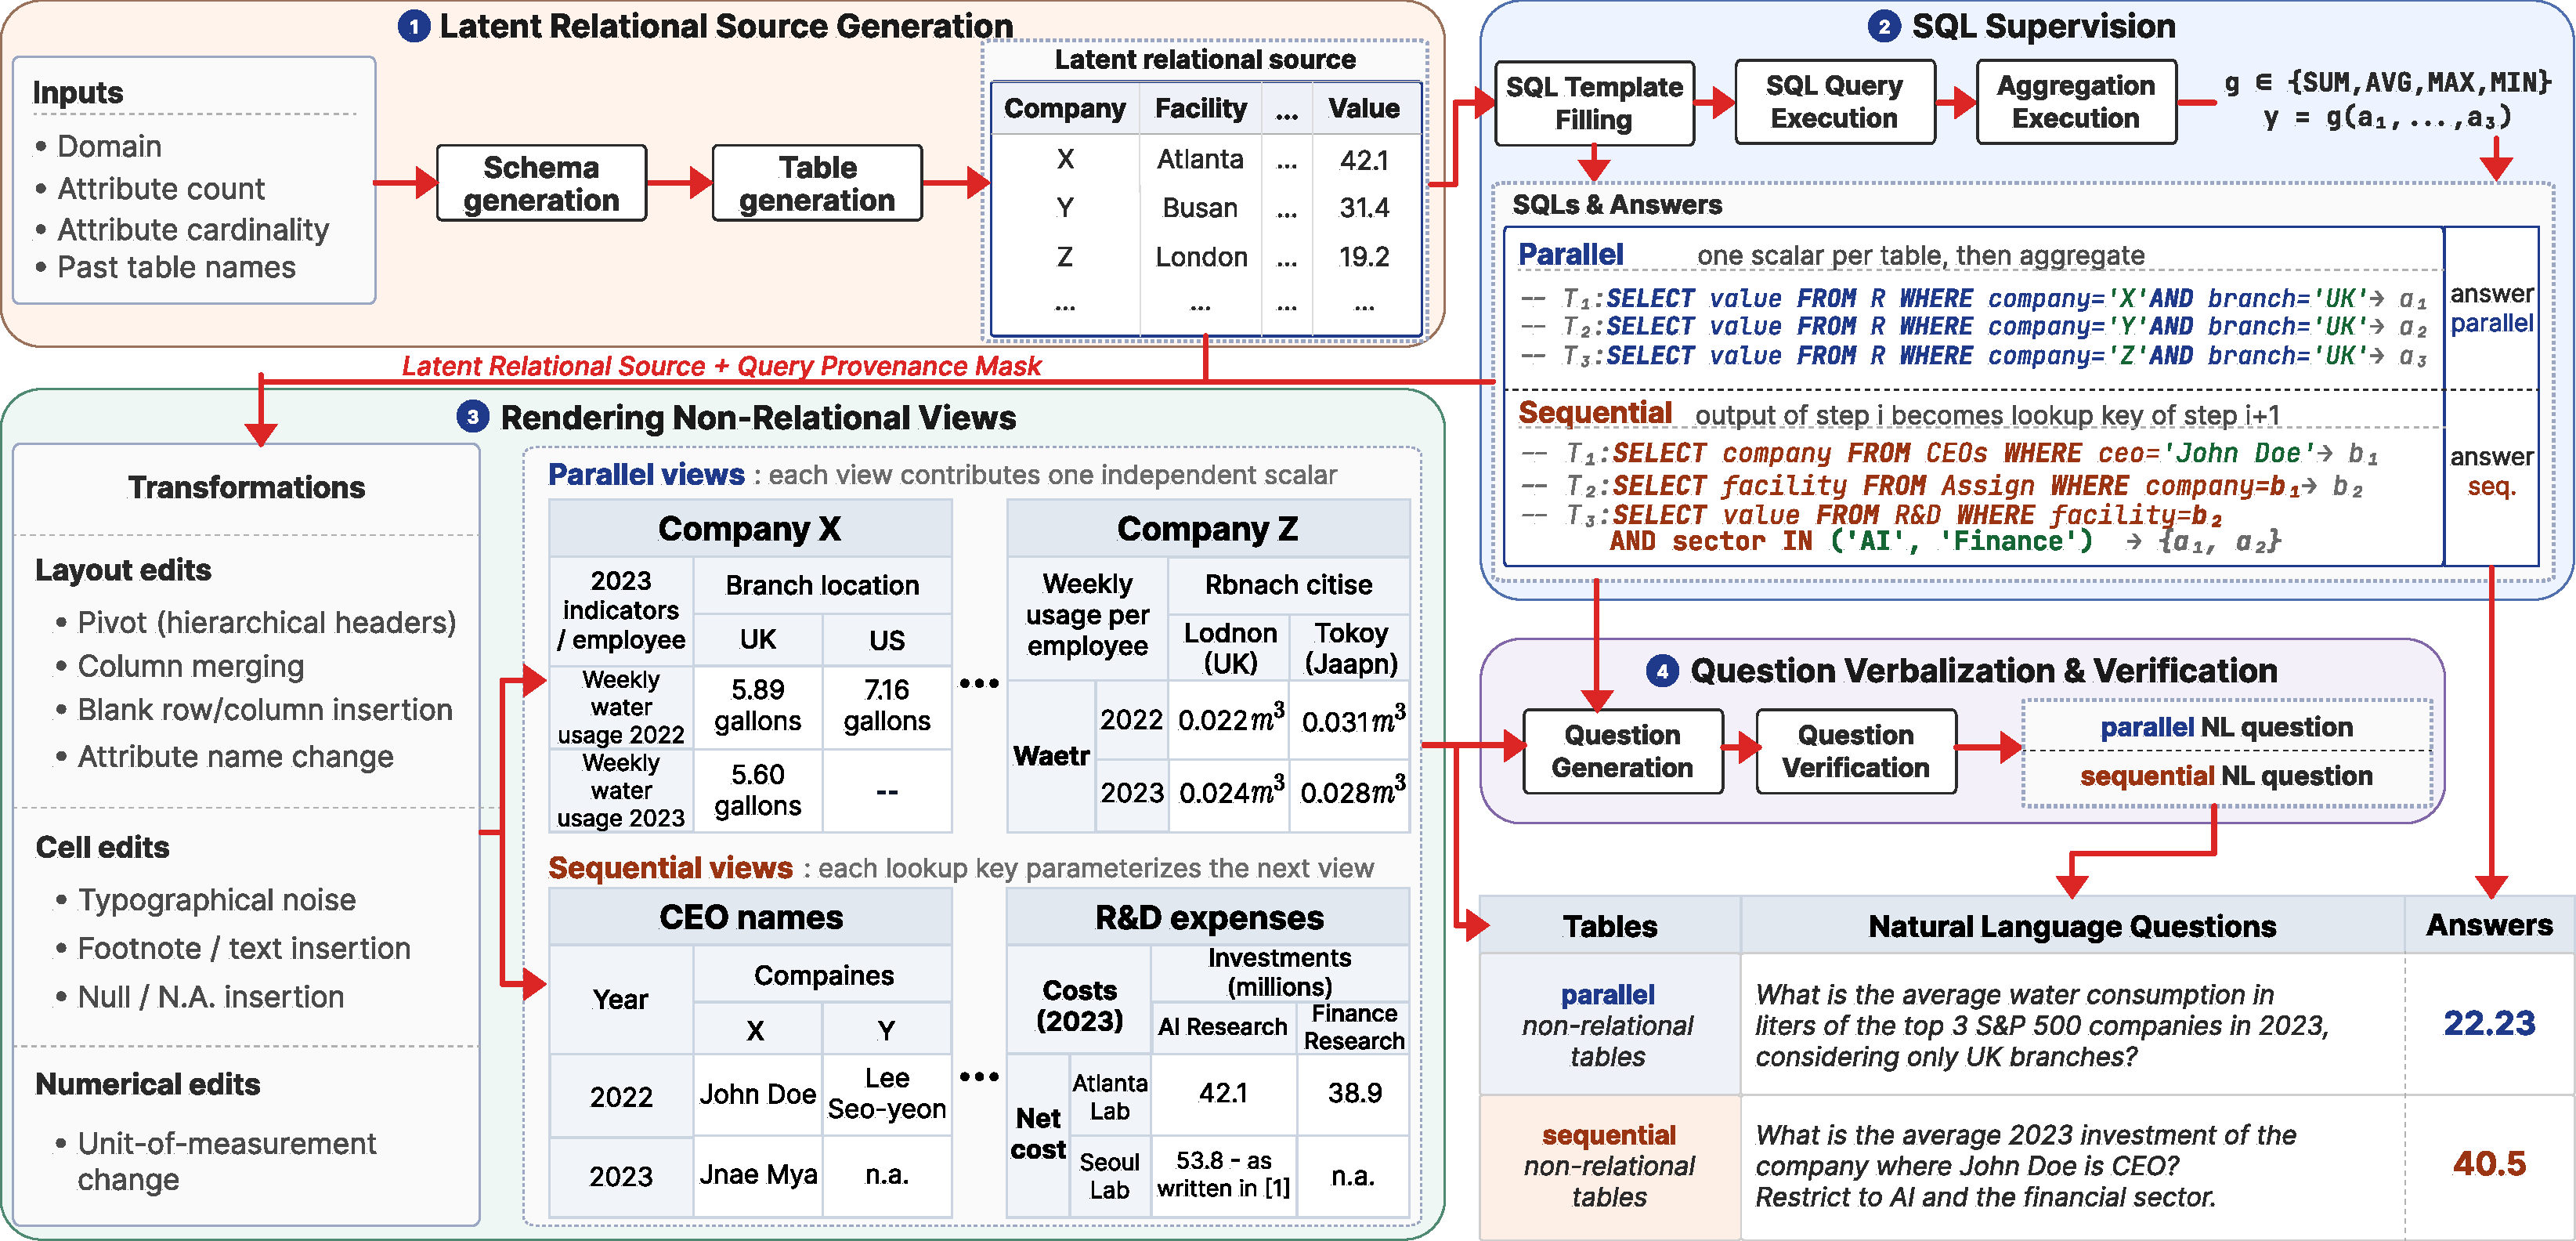
\includegraphics[width=\linewidth]{img/gradino.pdf}
    \caption{Overview of \name}
    \label{fig:pipeline}
    \vspace{-6pt}
\end{figure*}

\name\ generates automatically verifiable multi-table numerical QA instances over non-relational tables. Starting from a domain specification and a small set of generation controls, such as the number of attributes, their cardinalities, the number of tables to compose and their topic, \name\ first creates a clean relational source, then derives executable SQL supervision, next verbalizes the supervision into natural-language questions, and finally transforms the source into challenging non-relational multi-table inputs. This design decouples correctness from presentation: answers are computed on a controlled latent representation, while models are evaluated on noisy, heterogeneous tables.

\subsection{Data generation}
\label{subsec:data-generation}

\name\ begins by prompting an LLM to generate a plausible domain-specific schema, including attribute names, human-readable headers, attribute types, candidate value ranges, one distinguished numerical value attribute, and metadata about units of measurement. To steer generation toward realistic domains, we optionally condition the prompt on example tables and on domain-specific inventories of canonical units. Concretely, \name\ uses conversion resources derived from QUDT for environmental quantities and XBRL UTR for finance.

Given the schema, \name\ instantiates a dense relational table by enumerating combinations of non-value attributes and sampling the numerical field. To improve plausibility, the generator also samples lightweight semantic regularities over the table and enforces them during instantiation; these include row-level implications and cross-row numerical consistency conditions. We defer their exact formalization and solver implementation to Appendix~\ref{app:constraints}. The resulting table serves as the latent source from which all benchmark instances are derived.

For multi-table generation, \name\ does not sample unrelated tables independently. Instead, it derives several table views from the same source relation. This choice is important for two reasons. First, it preserves a known ground-truth correspondence between evidence pieces across tables. Second, it allows us to control the reasoning topology while keeping the final answer automatically verifiable.

\subsection{SQL Execution \& Multi-Table Generation}
\label{subsec:sql-execution}

From the latent relational source, \name\ samples executable SQL programs that define the target answer. In the multi-table setting, we focus on aggregation-style questions whose final answer is produced by combining scalar values extracted from different tables. At generation time, SQL therefore acts as an internal supervision language rather than as a user-facing formalism.

In the \textbf{parallel} setting, \name\ first samples a predicate template over a subset of non-value attributes that uniquely identifies one numerical value. It then instantiates multiple table-specific selections by varying exactly one attribute across tables while keeping the remaining predicate structure fixed. Each table contributes one scalar value $a_i$, and the final answer is computed by an aggregation operator
\begin{equation}
y = g(a_1,\dots,a_n), \qquad g \in \{\textsc{sum}, \textsc{avg}, \textsc{max}, \textsc{min}\}.
\end{equation}
Operationally, each table is associated with an extractive SQL query returning a single value, and the final label is obtained by applying the aggregation over the list of extracted scalars. This is the mechanism used to create multi-table sum, average, and superlative questions.

In the \textbf{sequential} setting, \name\ constructs a chain of table-local queries. Intermediate tables are associated with extractive queries whose returned value becomes the lookup key for the next table in the chain, while the final table applies the target numerical operation. Formally, if $b_1$ is extracted from $T_1$, then $b_1$ parameterizes the selection on $T_2$, whose output parameterizes the next step, and so on until the last table produces the value or values needed for the final aggregation. The gold label is the result of executing this latent composition. This setup yields multi-step reasoning across tables without relying on an externally given relational schema.

Because all SQL programs are executed on the clean source tables before perturbation, answer correctness is guaranteed by construction. Moreover, since the same latent source can be reused to generate multiple question types and different numbers of tables, the approach scales naturally across reasoning depths and evidence cardinalities.

\subsection{Natural-language generation}
\label{subsec:nl-generation}

Once the latent SQL program and its answer have been obtained, \name\ prompts an LLM to generate a natural-language question. The prompt receives the relevant tables in HTML form, the SQL supervision, the aggregation description, and the gold answer. The wording is therefore conditioned on the exact evidence and operation required by the instance.

The multi-table verbalization differs slightly across the two reasoning regimes. For parallel questions, the generator verbalizes the shared selection pattern together with the cross-table aggregation to be performed. For sequential questions, the generator verbalizes only the first and last steps of the chain and leaves intermediate dependencies implicit in the table contents. As a result, the final question does not expose the latent composition directly, but still requires the model to recover it from the tables. In both cases, the answer remains a scalar numerical value, except for some superlative cases where the target is the identifier associated with an extremal value.

To filter out noisy generations, we perform an LLM-based verification pass after question generation. The verifier receives the generated question, the supporting tables, the latent SQL program, and the gold answer, and rejects cases in which the verbalization is inconsistent with the underlying supervision. This step is especially important in the multi-table setting, where small deviations in phrasing can alter the intended evidence aggregation or composition.

\subsection{Transformations to non-relational multi-table inputs}
\label{subsec:transformations}

The final stage maps the clean relational source into the non-relational benchmark instance seen by the model. These transformations are designed to preserve the answer while increasing structural heterogeneity, layout complexity, and surface noise.

We first apply schema-level changes, such as replacing synthetic attribute names with longer web-style headers and optionally merging columns. We then render measurement units either in headers or directly inside cells. Next, we convert flat tables into non-relational layouts through a pivot-style transformation that organizes selected attributes as hierarchical row and column headers. The generator searches over candidate row/column partitions, prefers dense pivots, and shrinks the resulting layout while ensuring that all evidence cells required by the latent SQL program are retained. This is the main mechanism by which \name\ produces nested headers and non-trivial table layouts.

After layout construction, we apply cell- and structure-level perturbations, including blank rows and columns, null-like fillers in non-answer cells, typographical noise, and contextual or footnote-like text inserted into cells. Critically, the generator tracks answer-bearing cells throughout the pipeline and restores them whenever a perturbation would otherwise delete or corrupt the evidence needed to recover the gold label.

The same transformation machinery is used for both multi-table regimes, but the source-to-table mapping differs. In the parallel setting, each transformed table contains one independently retrievable scalar contribution to the final aggregation. In the sequential setting, each transformed table contains one step of a latent lookup chain, so that solving the question requires propagating information across tables before computing the final answer. In addition, for parallel generation \name\ can optionally apply unit conversion to some tables before perturbation, forcing models to normalize compatible quantities across heterogeneous surface forms. The converted values are accepted only when round-trip consistency can be maintained at the chosen decimal precision.

Overall, this transformation stage yields benchmark instances that no longer expose a clean relational schema, explicit joins, or standardized numerical expressions, while still remaining fully verifiable because every question is grounded in a latent source table and an executable supervision program. Additional details on perturbation types, constraint handling, and implementation choices are provided in the appendix.